\documentclass[12pt]{article}
\usepackage[utf8]{inputenc}
\usepackage{comment}
\usepackage{tabularx}
\usepackage[shortlabels]{enumitem}
\usepackage{amsmath}
\usepackage{amssymb}
\usepackage{mathtools}
\usepackage{graphicx}
\usepackage{caption}
\usepackage{subcaption}
\usepackage{hyperref}
\usepackage{xcolor}
\usepackage{pdflscape}
\usepackage[a4paper, margin=1.2cm]{geometry}
\hypersetup{
    colorlinks,
    linkcolor={red!50!black},
    citecolor={blue!50!black},
    urlcolor={blue!80!black}
}

\newtheorem{lemma}{Lemma}
\newtheorem{theorem}[lemma]{Theorem}
\newtheorem{prop}[lemma]{Proposition}
\newtheorem{cor}[lemma]{Corollary}
\newtheorem{assumption}[lemma]{Assumption}
\newtheorem{conj}{Conjecture}

\title{Notes on the training optimisation}
\author{Emma Ai}

\begin{document}
\maketitle
\section{The essential changes related to the model optimisation}

The optimisation of the GPT-2 style model proceeded through a sequence of targeted changes, each motivated by improving training stability, convergence, and generalisation performance. The key changes, their rationale, and the corresponding results are summarised below.


\subsection{Optimiser Adjustment}
\begin{itemize}
  \item \textbf{Change:} Replace \textit{SGD} with \textit{AdamW}.
  \item \textbf{Reasoning:} AdamW decouples weight decay from the gradient update and uses per-parameter adaptive learning rates, which improves convergence stability and generalisation over plain SGD. In GPT-2 style transformers, many parameters experience \emph{sparse or infrequent} updates (e.g., embeddings and attention projections on subpopulations of tokens); AdamW’s adaptive scaling handles such sparsity far better than SGD with a single global learning rate, while decoupled weight decay provides cleaner $L_2$ regularisation of dense and sparse weight vectors alike.
  \item \textbf{Results:} Validation loss was reduced to $1.4893$. The validation and training losses curves are shown in Fig.~\ref{fig:model_results}, run \texttt{mainrun\_2025-09-22T12-05-47.log}.
\end{itemize}


\subsection{Hyperparameter Tuning with Optuna}
\begin{itemize}
  \item \textbf{Change:} Introduce \textit{Optuna}~\cite{optuna} to sweep learning rate, dropout rate, and block size.  
  \item \textbf{Additional Setting:} $weight\_decay=0.01$ in AdamW.
  \item \textbf{Reasoning:} Automated search provides systematic exploration of hyperparameters that strongly affect overfitting and stability. The implementation leveraged the official Optuna GitHub repository: \url{https://github.com/optuna/optuna}.
  \item \textbf{Results:} Validation loss was reduced to $1.3544$ with the set hyperparameters after tuning. The validation and training losses curves are shown in Fig.~\ref{fig:model_results},  run \texttt{mainrun\_2025-09-23T03-25-45.log}.
\end{itemize}

\subsection{Sharpness-Aware Minimisation (SAM) and Warm-Up}
\begin{itemize}
  \item \textbf{Change:} Add SAM optimiser~\cite{sam} and introduce learning-rate warm-up schedule.
  \item \textbf{Reasoning:} SAM encourages flatter minima and improved generalisation; warm-up stabilises early training. The PyTorch implementation \url{https://github.com/davda54/sam} is used.
  \item \textbf{Results:} Validation loss was reduced to $1.327$ with the set of hyperparameters after tuning. The validation and training losses curves are shown in Fig.~\ref{fig:model_results},  run \texttt{mainrun\_2025-09-23T08-09-24.log}.
\end{itemize}

\subsection{Adaptive SAM}
\begin{itemize}
  \item \textbf{Change:} Replace standard SAM with adaptive SAM~\cite{asam}.
  \item \textbf{Reasoning:} Adaptive SAM adjusts perturbations based on parameter magnitudes, yielding better scaling for deep networks, specifically for large language models (LLMs) where weight vector scales can vary substantially across layers. The PyTorch implementation \url{https://github.com/davda54/sam} is used.
  \item \textbf{Results:} Validation loss was reduced to $1.311$ with the same set of hyperparameters as SAM. The validation and training losses curves are shown in Fig.~\ref{fig:model_results},  run \texttt{mainrun\_2025-09-23T09-36-58.log}.
\end{itemize}

\subsection{Model Size Reduction (Phase I)}
\begin{itemize}
  \item \textbf{Change:} Reduce model size: $vocab\_size = 4\text{K}, n\_head = 6, d\_model = 384$.
  \item \textbf{Additional Setting:} Exclude weight decay for bias, norm, and embedding layers. Plato minimum learning rate at $1\times 10^{-5}$.
  \item \textbf{Reasoning:} The training corpus contains only $\sim\!1.1\,\mathrm{M}$ tokens. Smaller models reduce capacity (mitigating overfitting on limited data) and lower computational load. Excluding weight decay for bias, LayerNorm, and embedding parameters preserves scale-sensitive statistics and representational capacity.
  \item \textbf{Results:} Validation loss was reduced to $1.2935$ with the set of hyperparameters after tuning. The validation and training losses curves are shown in Fig.~\ref{fig:model_results},  run\texttt{mainrun\_2025-09-24T08-55-04.log}.
\end{itemize}

\subsection{Model Size Reduction (Phase II)}
\begin{itemize}
  \item \textbf{Change:} Further reduce depth and width: $n\_layer = 4, n\_head = 3, d\_model = 192$.
  \item \textbf{Reasoning:} Experiment with lightweight configurations to test lower bounds of model capacity while retaining stable training.
  \item \textbf{Results:} Validation loss was increased to $1.3206$ with the set of hyperparameters after tuning.  The validation and training losses curves are shown in Fig.~\ref{fig:model_results},  run \texttt{mainrun\_2025-09-24T09-27-54.log}.
\end{itemize}

\paragraph{Held-out evaluation on in-domain titles.}
The two reduced-size models were evaluated on $20{,}000$ titles held out from the same corpus (not used in training). The results are on par with validation performance; perplexity is reported as $\mathrm{ppl}=\exp(\text{loss})$.

\begin{table}[h]
\centering
\label{tab:heldout_eval}
\caption{Held-out results on $20{,}000$ in-domain titles.}
\begin{tabular}{lcc}
\textbf{Checkpoint} & \textbf{Loss} & \textbf{Perplexity} \\
\texttt{models/model\_midsize.pth}  & 1.3021 & 3.6771 \\
\texttt{models/model\_smallsize.pth} & 1.3302 & 3.7816 \\
\end{tabular}
\end{table}

\begin{landscape}
\begin{figure}[ht!]
	\caption{GPT-2 Model Optimisation Experiments}
	\centering
	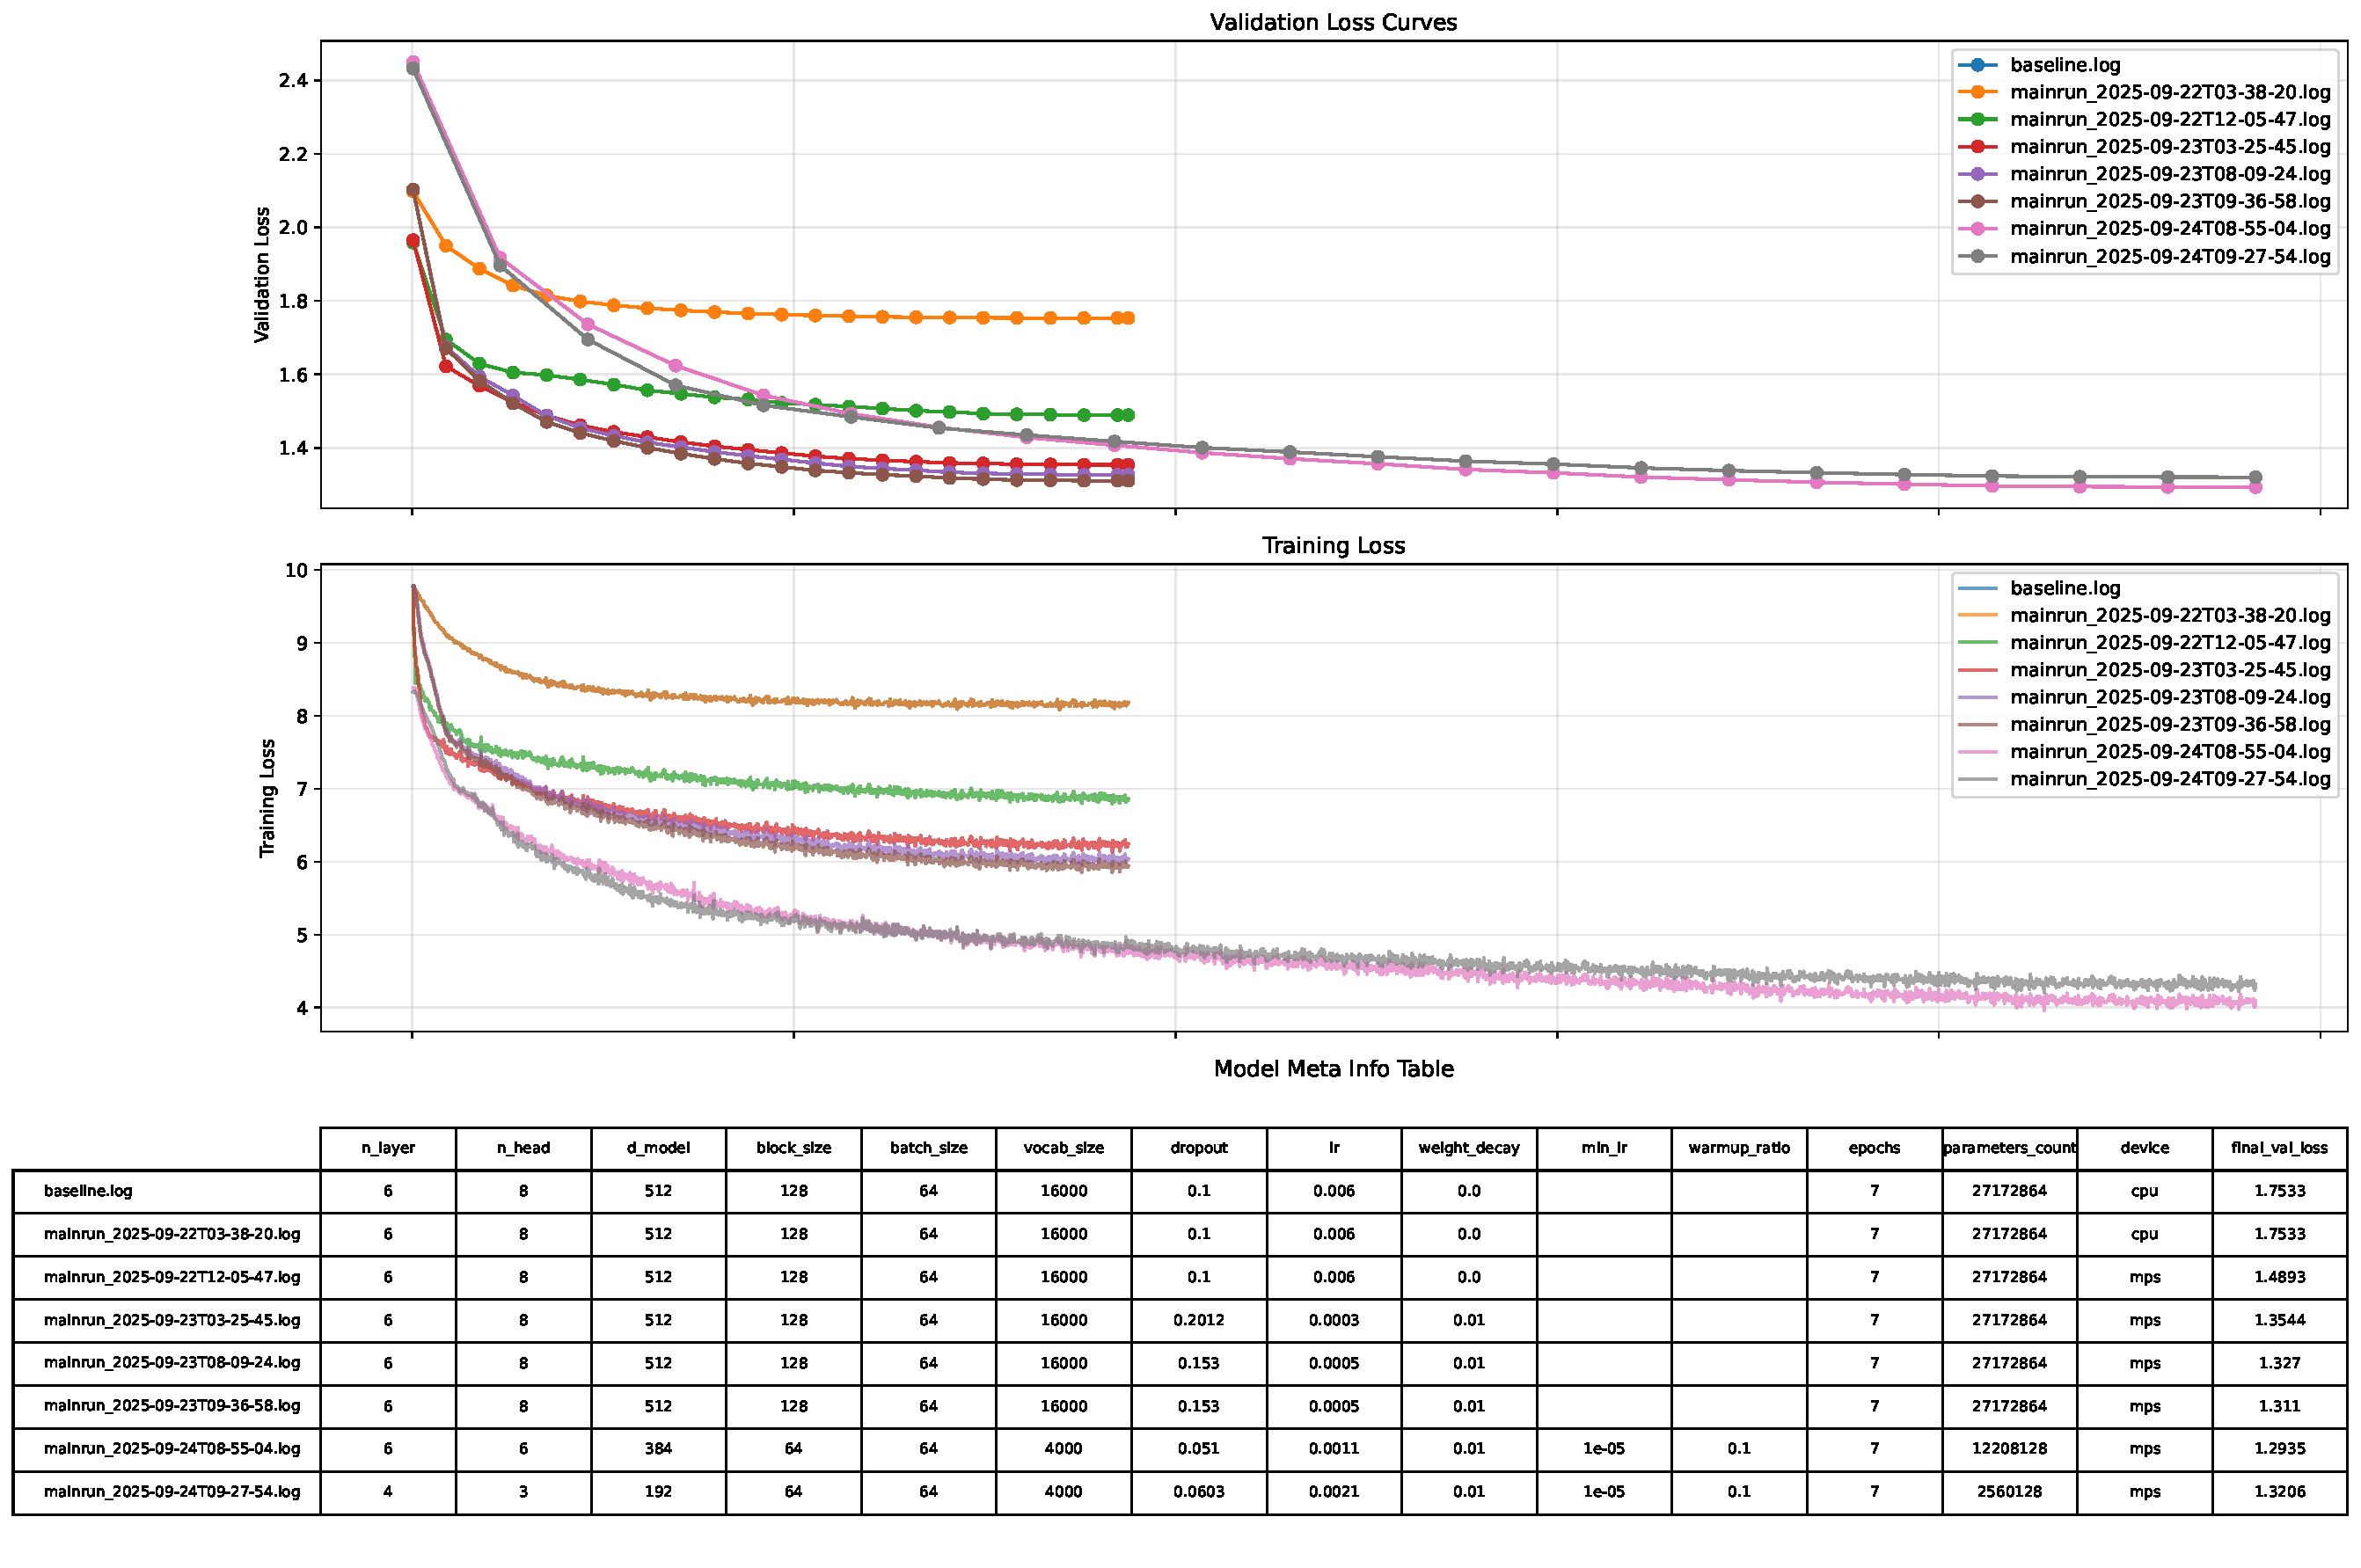
\includegraphics[scale=.6]{model_plot.pdf}
	\label{fig:model_results}
\end{figure}
\end{landscape}

\section{The other essential code and configurations}


\begin{itemize}
  \item \texttt{helper.py}: Utilities to plot the model \emph{architecture} and diagnose \emph{tokeniser} efficiency (coverage, OOV rate, length stats).
  \item \texttt{model\_analysis.py}: Reproduces Fig.~\ref{fig:model_results} (training/validation loss curves, run annotations).
  \item \texttt{model\_evaluate.py}: Evaluates saved checkpoints on held-out data and reports loss/perplexity tables.
  \item \texttt{train\_config.yaml}: Experiment configuration (model hyperparameters, tune/train, hyperparameter DB and model saving path).
  \item \texttt{hyperparameter.db}: \textsc{SQLite} database (Optuna study) tracking trials, sampled hyperparameters, and best scores.
  \item \texttt{hptune.sh}: A simple shell to run $N$ trials.
\end{itemize}

The full codebase including running environment (updated docker file and \texttt{docker\_compose.yml}) to replicate these experiments is in repo \url{https://github.com/emmaai/mainrun}.

\bibliographystyle{plain}
\bibliography{refs}
\end{document}
